% 实验1 机械臂运动控制仿真 实验报告（LaTeX 版）
% 编译：xelatex report.tex；导出 Word：pandoc report.tex -o report_latex.docx
\documentclass[11pt,a4paper]{ctexart}
\usepackage{amsmath,amssymb,bm}
\usepackage{graphicx}
\usepackage[margin=2.5cm]{geometry}
\usepackage{booktabs}
\usepackage{caption}
\usepackage{hyperref}
\graphicspath{{figures/}}
\captionsetup{font=small,labelsep=quad}

\begin{document}

% ==================== 封面 ====================
\begin{titlepage}
  \centering
  {\large 组号：\underline{\hspace{4em}}}\hfill\mbox{}\par
  \vspace{5cm}
  {\Huge\bfseries 本科实验报告}\par
  \vspace{2.5cm}
  {\large
  \begin{tabular}{ll}
    课程名称： & \underline{\makebox[16em]{机器人与智能系统综合实践}}\\[1ex]
    姓\hspace{2em}名： & \underline{\makebox[16em]{}}\\[1ex]
    院\hspace{2em}系： & \underline{\makebox[16em]{}}\\[1ex]
    专\hspace{2em}业： & \underline{\makebox[16em]{}}\\[1ex]
    学\hspace{2em}号： & \underline{\makebox[16em]{}}\\[1ex]
    指导老师： & \underline{\makebox[16em]{}}\\[1ex]
    选课时间： & \underline{\makebox[16em]{}}\\
  \end{tabular}\par}
  \vfill
  {\large \hspace{2em}年\hspace{2em}月\hspace{2em}日}
\end{titlepage}

\section{实验目的和要求}

\subsection{实验目的}
掌握并灵活运用关节型机械臂运动控制相关理论和知识，解决一般构型机械臂的运动控制问题。

\subsection{实验要求}
以中国空间站太空机械臂为仿真对象，设计开发机械臂控制算法和程序，在仿真环境中演示该机械臂在空间站上移动和行走。具体包括：
\begin{enumerate}
  \item 根据缩小版的机械臂结构和尺寸，利用 DH 方法\textbf{正运动学建模}；
  \item 分析并给出该机械臂的\textbf{逆运动学解析解}；
  \item 采用一种\textbf{轨迹规划方法}，控制该机械臂在空间站上行走，至少行走 2 步，即从初始位置移动到位置 1，再移动到位置 2，运动时速度在合理范围内自定义，保证速度、加速度连续；
  \item 假设机械臂末端与基座之间接触后可以通过电磁铁紧密吸合，借助仿真环境进行\textbf{可视化演示}。
\end{enumerate}

\section{主要仪器}
CoppeliaSim + Python（ZeroMQ Remote API）。

\section{实验内容和原理}

\subsection{D-H 参数表}
机械臂为 7 自由度对称构型（关节轴依次为 Z-Y-X-X-X-Y-Z），两端均为可与基座电磁吸合的末端。以左足（\texttt{L\_Base}）落足面为基坐标系 $\{0\}$（$z_0$ 垂直于落足面向外），沿链路到右足（\texttt{R\_Base}）建立各关节坐标系，按标准 D-H 方法（$z_i$ 沿关节 $i{+}1$ 轴线）测得参数如表~\ref{tab:dh} 所示。

\begin{table}[htbp]
  \centering
  \caption{机械臂 D-H 参数（长度单位 mm，角度单位 $^\circ$）}
  \label{tab:dh}
  \begin{tabular}{ccccc}
    \toprule
    $i$ & $a_{i-1}$/mm & $\alpha_{i-1}$/$^\circ$ & $d_i$/mm & $\theta_i$\\
    \midrule
    1 & 0   & 0   & 65   & $\theta_1$\\
    2 & 0   & 90  & 50   & $\theta_2$\\
    3 & 0   & 90  & 50   & $\theta_3$\\
    4 & 400 & 0   & 100  & $\theta_4$\\
    5 & 400 & 180 & 100  & $\theta_5$\\
    6 & 0   & 90  & $-50$ & $\theta_6$\\
    7 & 0   & 90  & $-50$ & $\theta_7$\\
    末端 & 0 & 0  & 65   & ---\\
    \bottomrule
  \end{tabular}
\end{table}

\subsection{正运动学求解与推导过程}
每个关节绕自身 $z$ 轴旋转，相邻坐标系之间的变换为常值矩阵 $A_i$（由零位测量得到）。正运动学为齐次变换连乘：
\begin{equation}
  {}^{0}T_{7} = A_0\,R_z(\theta_1)\,A_1\,R_z(\theta_2)\,A_2\,R_z(\theta_3)\,A_3\,R_z(\theta_4)\,A_4\,R_z(\theta_5)\,A_5\,R_z(\theta_6)\,A_6\,R_z(\theta_7)\,A_7,
\end{equation}
其中 $R_z(\theta)$ 为绕 $z$ 轴的旋转矩阵，$A_i$ 由表~\ref{tab:dh} 的 D-H 参数确定：
\begin{equation}
  A_i = \mathrm{Trans}(z, d_i)\,\mathrm{Rot}(x, \alpha_i)\,\mathrm{Trans}(x, a_i).
\end{equation}
程序实现见 \texttt{src/kinematics.py} 的 \texttt{fk()}。经验证：零位 $\theta=0$ 时正运动学给出的右足位姿 $(0.35,\,0,\,0.235)$ 与仿真场景中 \texttt{R\_Base} 的实际位姿完全一致（误差 $<10^{-6}$~m）。

\subsection{逆运动学解析解推导过程}
行走时支撑足固定于落足盘、摆动足需到达给定位姿，7 自由度存在 1 个冗余自由度。取矢状面（$x$--$z$ 平面）行走位形族并用``对称拱形''条件消解冗余：
\begin{enumerate}
  \item 令 $\theta_1=\theta_7=0$，机械臂保持在 $y=0$ 平面内；
  \item 中间三个平行俯仰关节取 $\theta_3=t$，$\theta_4=\pi-2t$，$\theta_5=\pi-t$。此时三关节簇的净转角为 0（末端姿态不受影响），且其在 $y$ 方向的位移相互抵消，两肩关节之间形成一根``虚拟连杆'' $\bm{v}=(-L,\,h)$，其中 $L=300$~mm 为固定轴向距离，$h=2l\cos t$（$l=400$~mm 为长臂杆长度）；
  \item 设目标摆动足相对支撑足的偏移为 $(D,\,\Delta z)$（足面法线保持竖直），令 $r^2=D^2+\Delta z^2$，则解析解为
  \begin{align}
    h &= \sqrt{r^2-L^2}, & t &= \arccos\!\left(\frac{h}{2l}\right),\\
    \theta_2 &= \operatorname{atan2}(\Delta z,\,D)-\operatorname{atan2}(h,\,-L), & \theta_6 &= -\theta_2.
  \end{align}
\end{enumerate}
可解性条件为 $L\le r\le\sqrt{L^2+4l^2}$，即 $0.3~\text{m}\le r\le 0.906~\text{m}$；第 1 步（$D=0.6$~m）满足该条件。位置 2 位于侧面落足盘（法线沿 $+y$，需三维姿态变换），此时在解析解给出的初值附近用基于解析雅可比矩阵的阻尼最小二乘法迭代求精（\texttt{src/kinematics.py} 的 \texttt{ik\_numeric()}），数步内收敛到 $10^{-6}$。

此外，$\theta_3=\theta_5=s$、$\theta_4=0$（$\theta_1=\theta_2=\theta_6=\theta_7=0$）为保持两足位姿不变的自运动族，用于起步前从零位平滑过渡到拱形位形族（$s\colon 0\to\pi/2$）。

\subsection{轨迹规划方法}
采用关节空间分段五次多项式（quintic）轨迹。相邻路径点之间使用归一化时间标度
\begin{equation}
  s(\tau)=10\tau^3-15\tau^4+6\tau^5,\qquad \tau\in[0,1],
\end{equation}
其一、二阶导数在两端均为零，因此整条轨迹的关节位置、速度、加速度全程连续，且吸合/脱开瞬间速度与加速度为零，满足电磁铁吸合的平稳性要求。

路径点由逆运动学求得：第 1 步（左足 $0.65$~m $\to$ 位置 1（$-0.25$~m 顶部落足盘），以右足为支撑）共 7 个路径点（含自运动过渡、抬升、越过支撑足、下落吸合），历时 14~s；第 2 步（右足 $0.35$~m $\to$ 位置 2（$-0.65$~m 侧面落足盘，法线沿 $+y$），以左足为支撑）共 7 个路径点（抬升、沿舱体上方平移、在舱体上方转入侧面姿态、沿侧面落足盘 $+y$ 法线逐段逼近并吸合），历时 13~s。实现见 \texttt{src/trajectory.py} 与 \texttt{src/walk.py}。

行走通过``基座交换''实现：第 1 步中右足固定，运动学树根（\texttt{L\_Base}）按 $T_L = T_R^{\text{fixed}}\,\bigl({}^{0}T_{7}(q)\bigr)^{-1}$ 浮动更新；第 2 步左足（树根）固定，直接驱动关节。

\section{实验结果说明与分析}
仿真在 CoppeliaSim 4.7（ZeroMQ Remote API + Python）中完成。机械臂从初始位置（两足位于 $x=0.65$~m 与 $0.35$~m 顶部落足盘）出发，第 1 步左足吸合到位置 1（$x=-0.25$~m 顶部落足盘），第 2 步右足吸合到位置 2（$x=-0.65$~m 侧面落足盘），完成 2 步行走。终点位姿误差为 0：左足 $(-0.25,\,0,\,0.235)$，右足 $(-0.65,\,0.1325,\,0.101)$，均与落足盘理论位姿一致。

全程关节速度峰值约 $4.4$~rad/s、加速度峰值约 $5.5$~rad/s$^2$，速度与加速度曲线连续无跳变（图~\ref{fig:curves}），足端在吸合与脱开时刻速度、加速度为零；第 1 步中两足始终保持在 $y=0$ 平面内，第 2 步足端法线由 $+z$ 平滑翻转到 $+y$。

第 2 步路径考虑了与舱体（半径约 $0.134$~m 的圆柱）的避碰：每个路径点在碰撞检测下选取无碰撞的逆解分支（\texttt{src/plan\_step2.py}），足端在舱体上方转入侧面落足盘姿态后沿其 $+y$ 法线方向逐步逼近，臂杆自然绕过舱体侧面（图~\ref{fig:step2swing}、图~\ref{fig:step2dock}）；对整条五次多项式轨迹按 400 个采样点密集校验，各连杆与舱体表面的最小间隙全程非负，无穿透。

\begin{figure}[htbp]
  \centering
  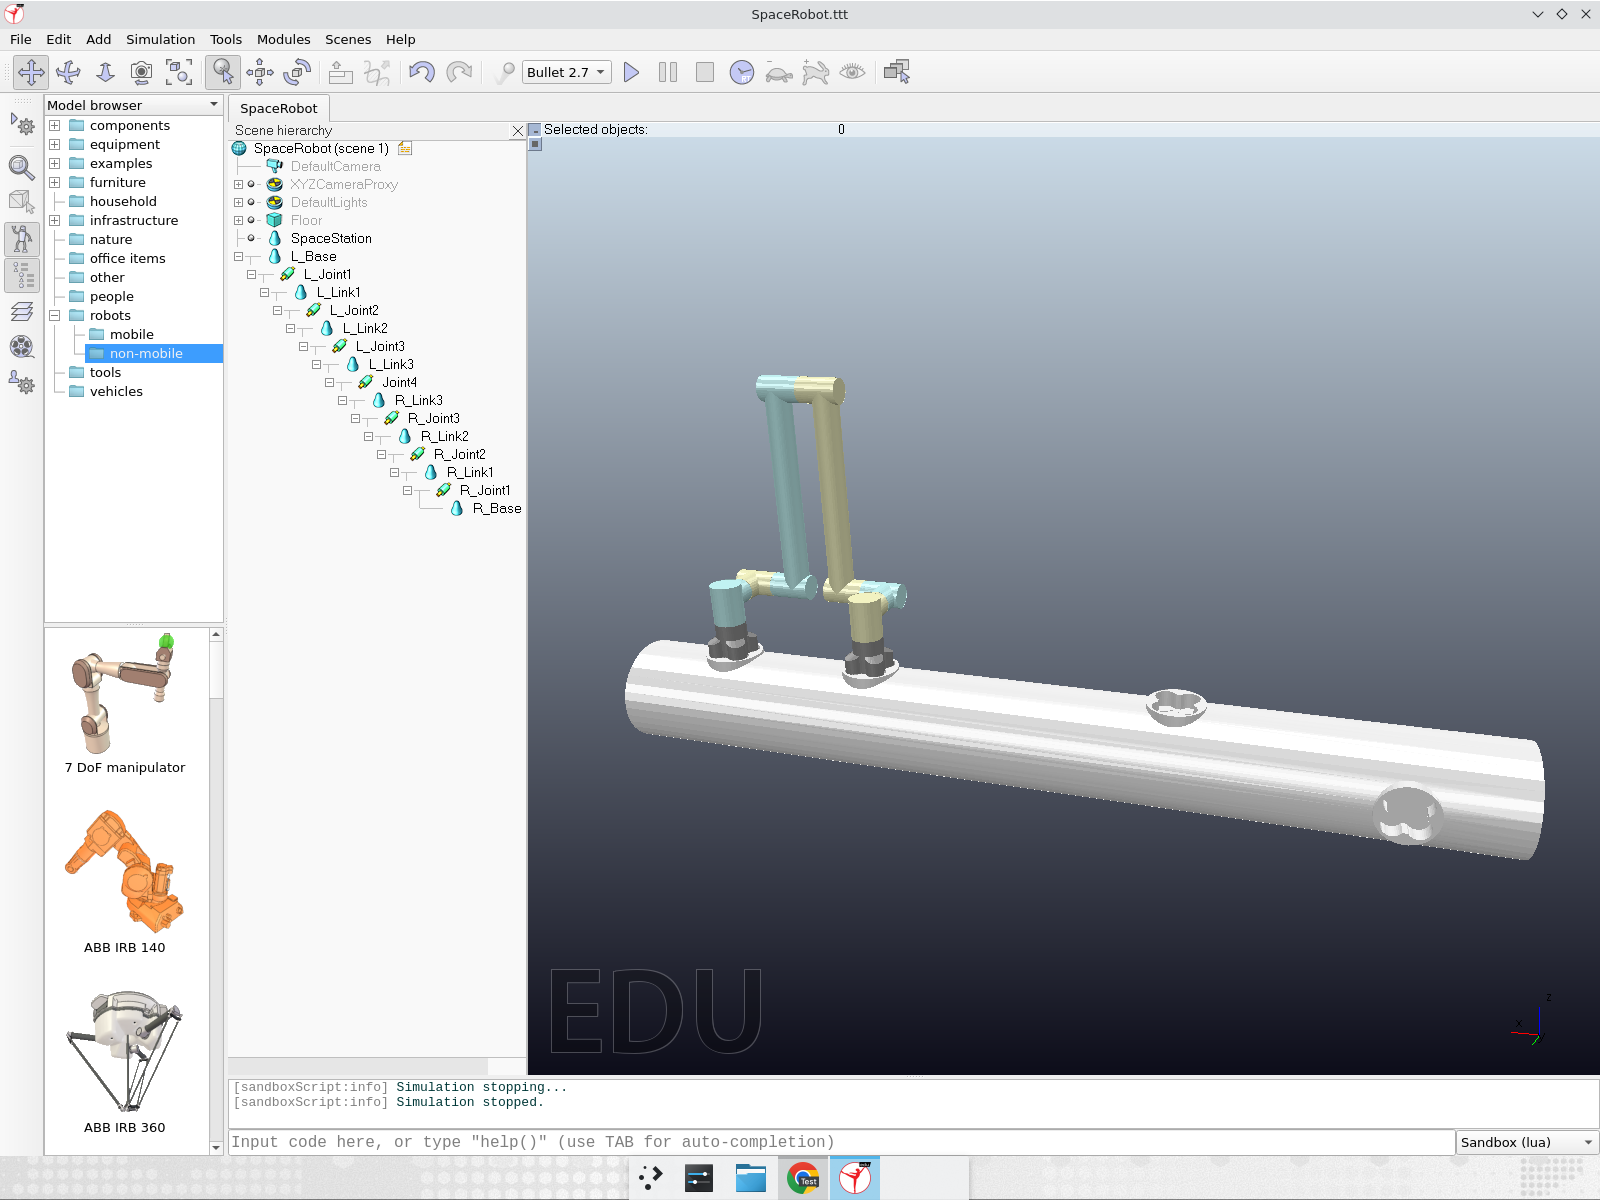
\includegraphics[width=0.8\textwidth]{initial_pose.png}
  \caption{初始位形（场景总览，两足位于顶部落足盘）}
  \label{fig:init}
\end{figure}

\begin{figure}[htbp]
  \centering
  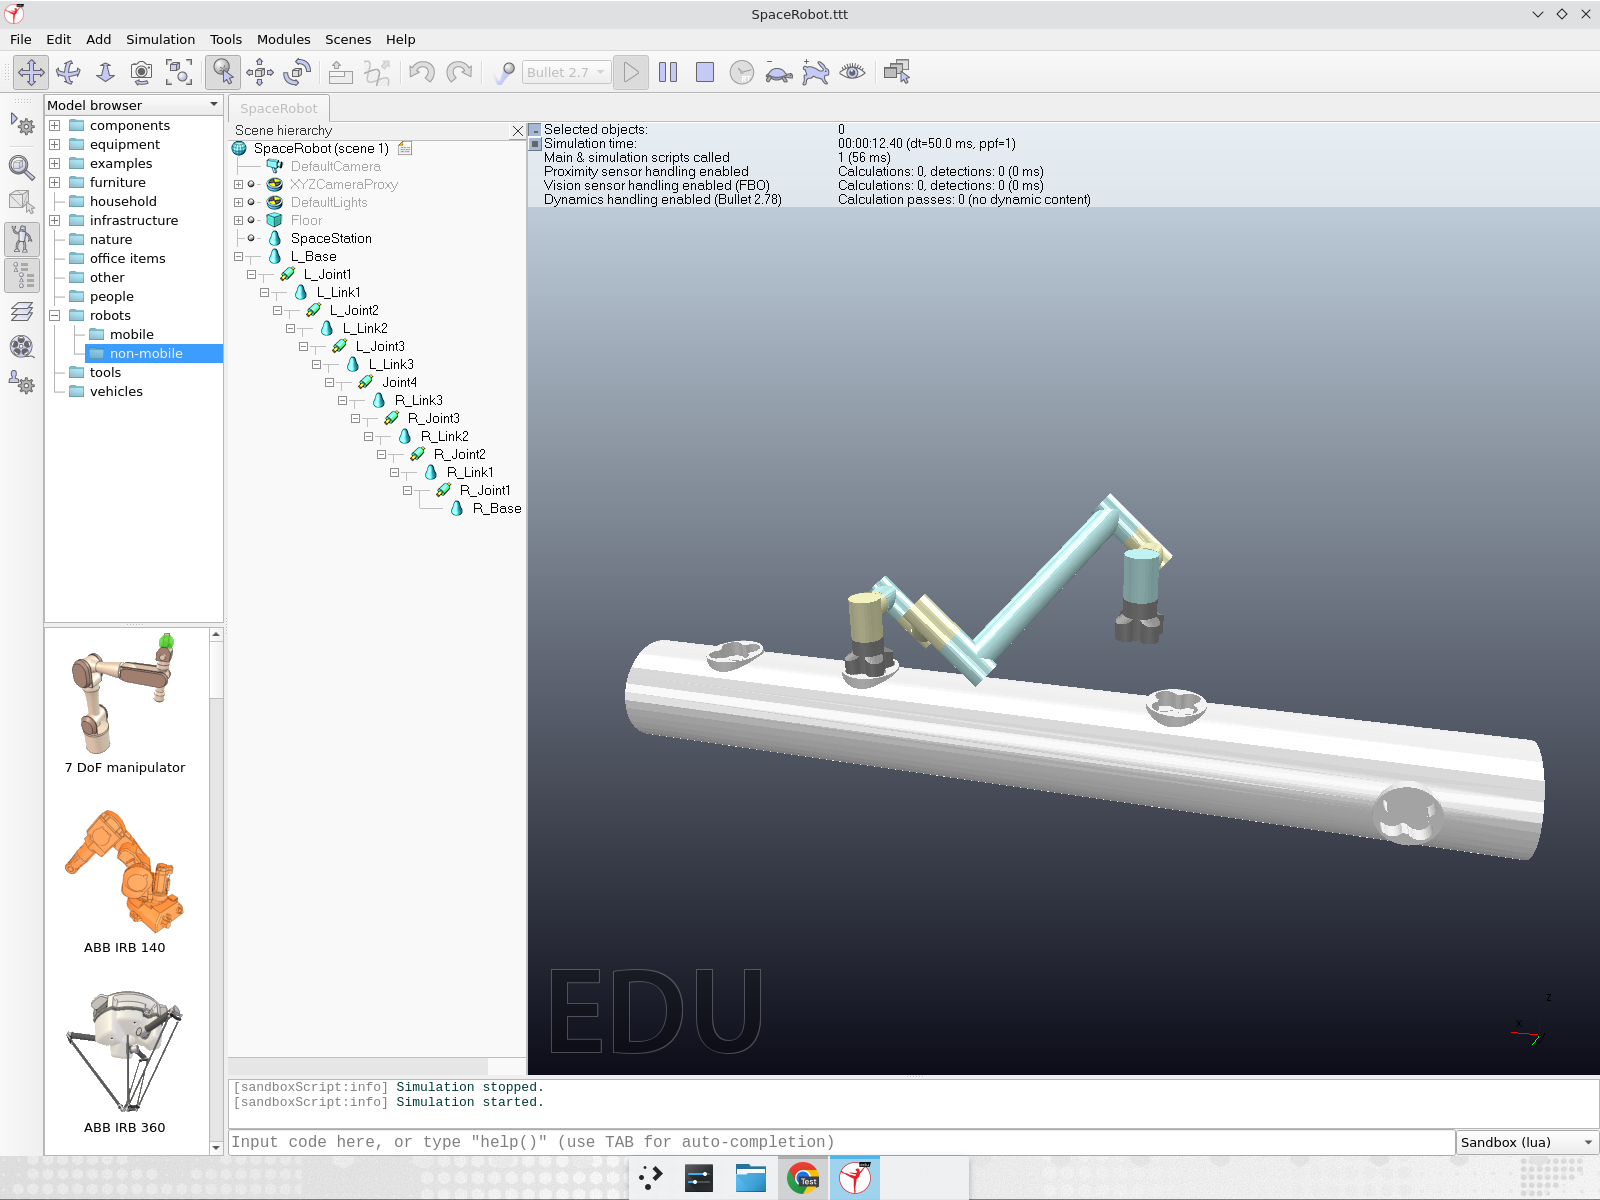
\includegraphics[width=0.8\textwidth]{step1_swing.png}
  \caption{第 1 步摆动过程（左足越过支撑足摆向位置 1）}
  \label{fig:step1}
\end{figure}

\begin{figure}[htbp]
  \centering
  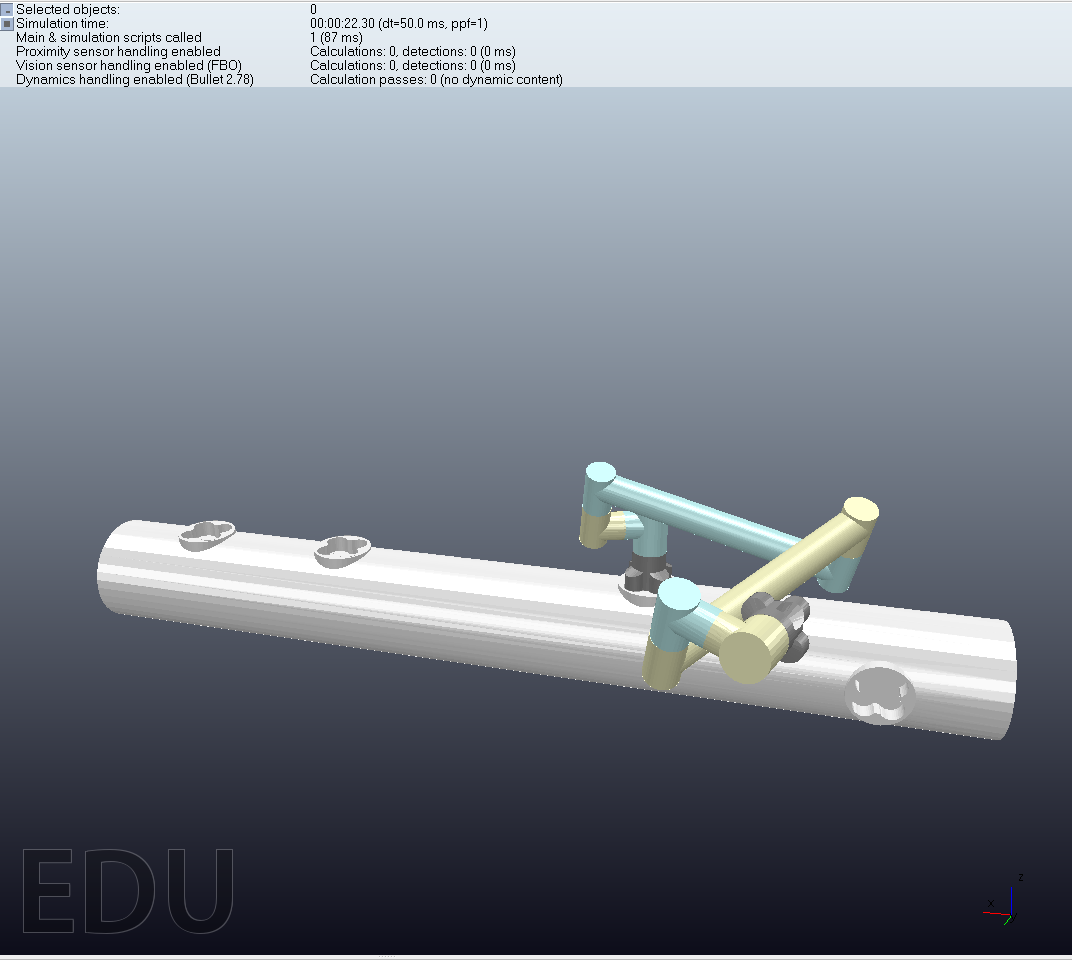
\includegraphics[width=0.8\textwidth]{step2_swing.png}
  \caption{第 2 步摆动过程（右足在舱体上方转入侧面姿态）}
  \label{fig:step2swing}
\end{figure}

\begin{figure}[htbp]
  \centering
  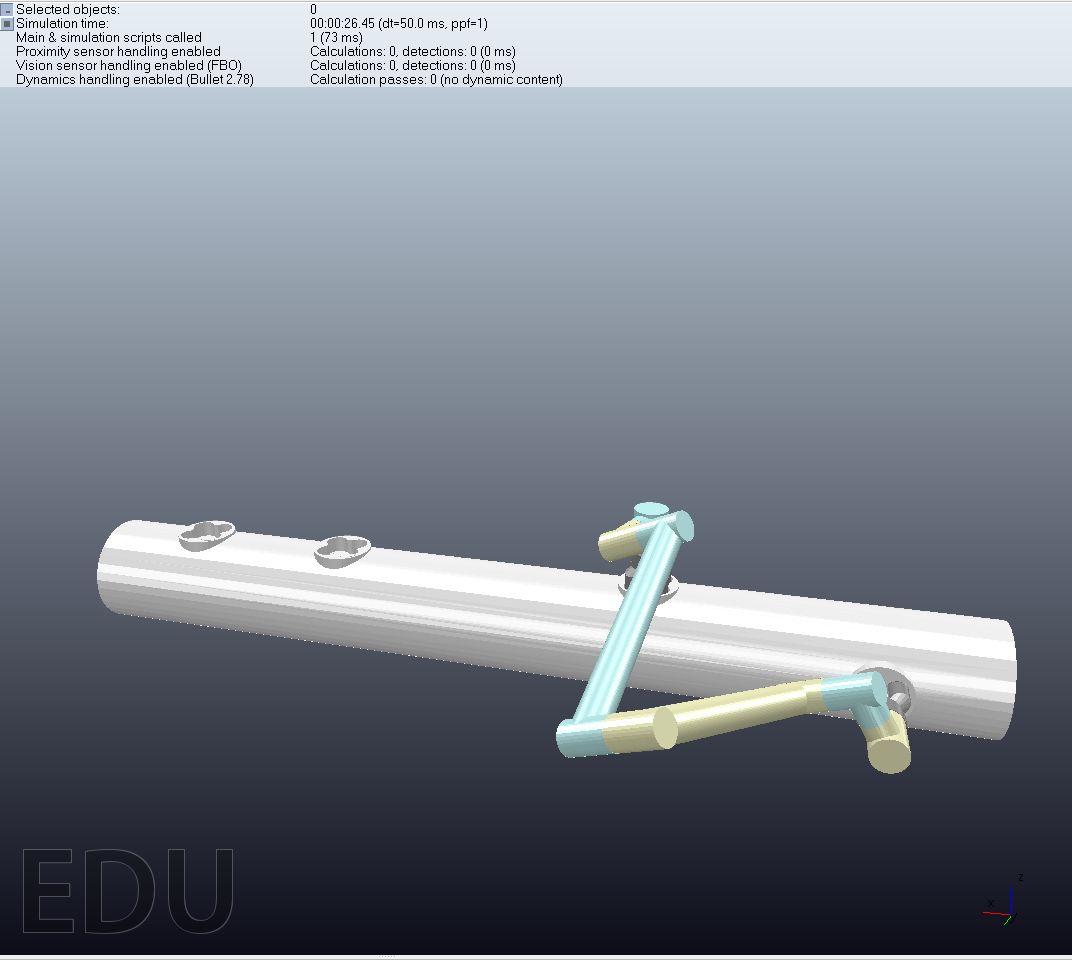
\includegraphics[width=0.8\textwidth]{step2_dock.png}
  \caption{第 2 步沿侧面落足盘 $+y$ 法线逼近（臂杆绕过舱体，无穿透）}
  \label{fig:step2dock}
\end{figure}

\begin{figure}[htbp]
  \centering
  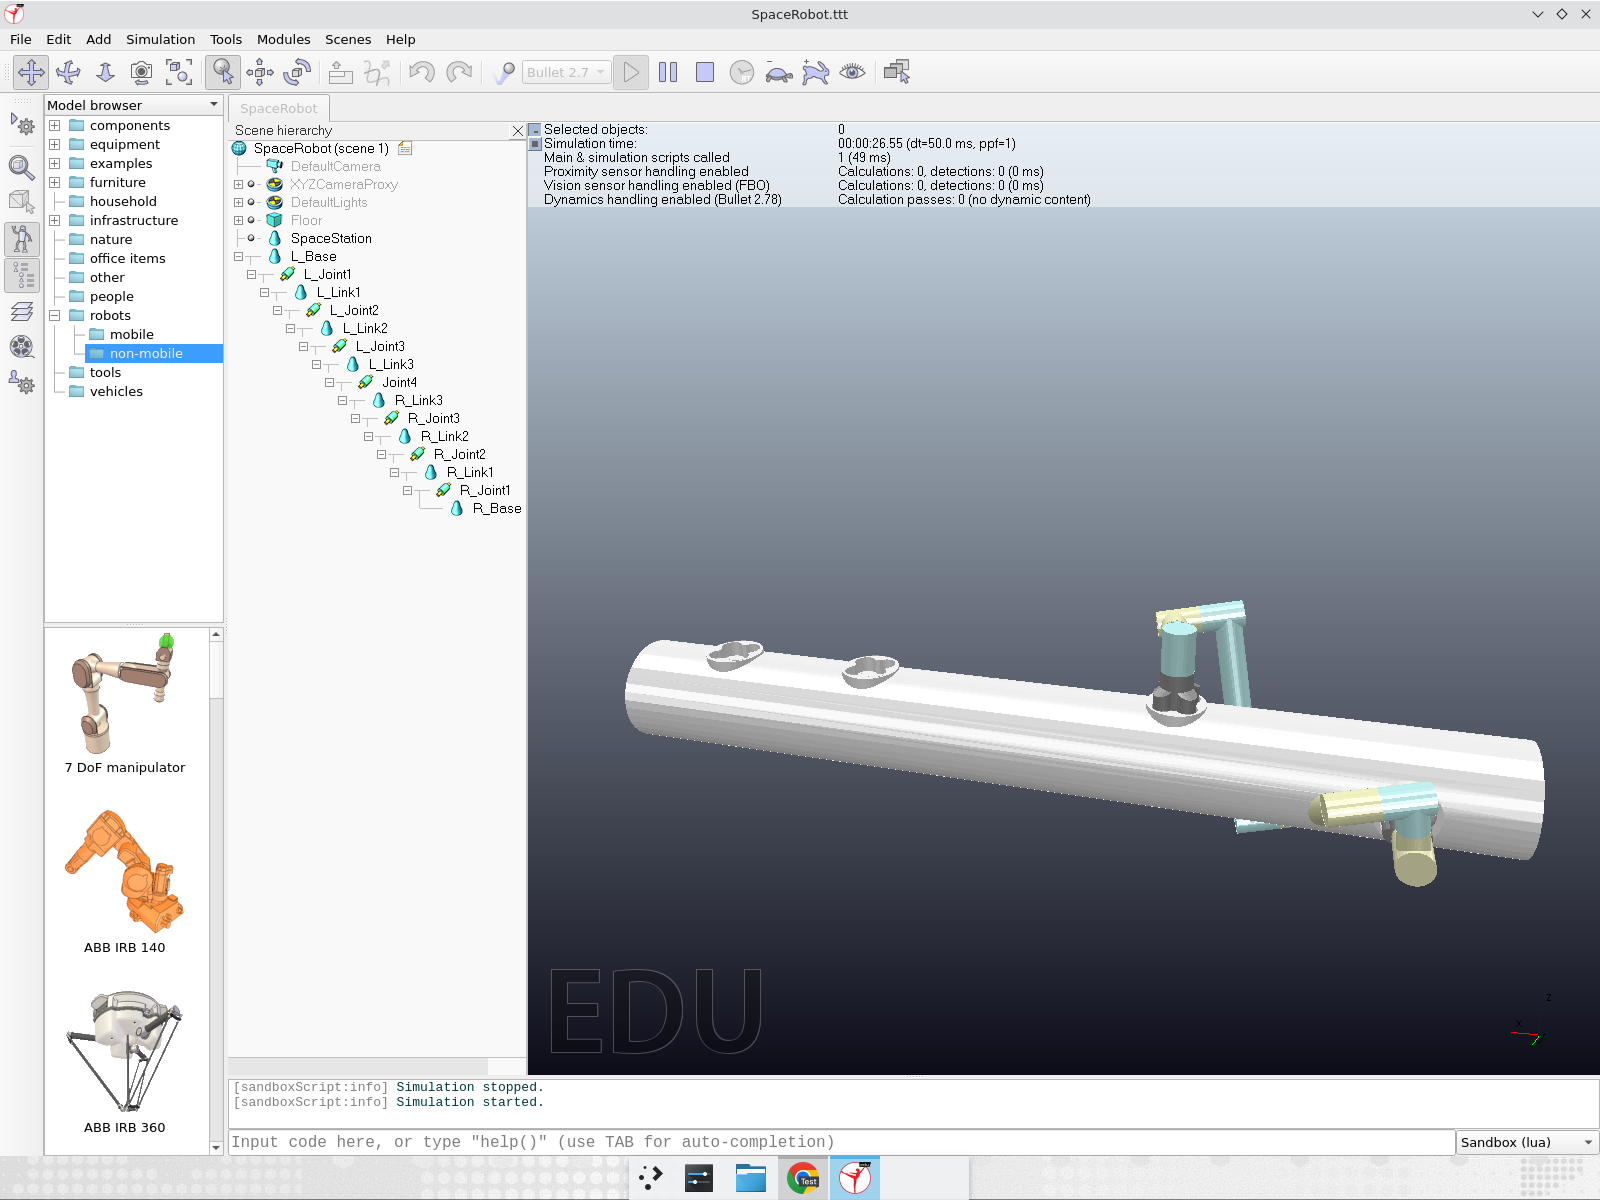
\includegraphics[width=0.8\textwidth]{final_docked.png}
  \caption{行走完成（左足位于位置 1，右足吸合于侧面位置 2）}
  \label{fig:final}
\end{figure}

\begin{figure}[htbp]
  \centering
  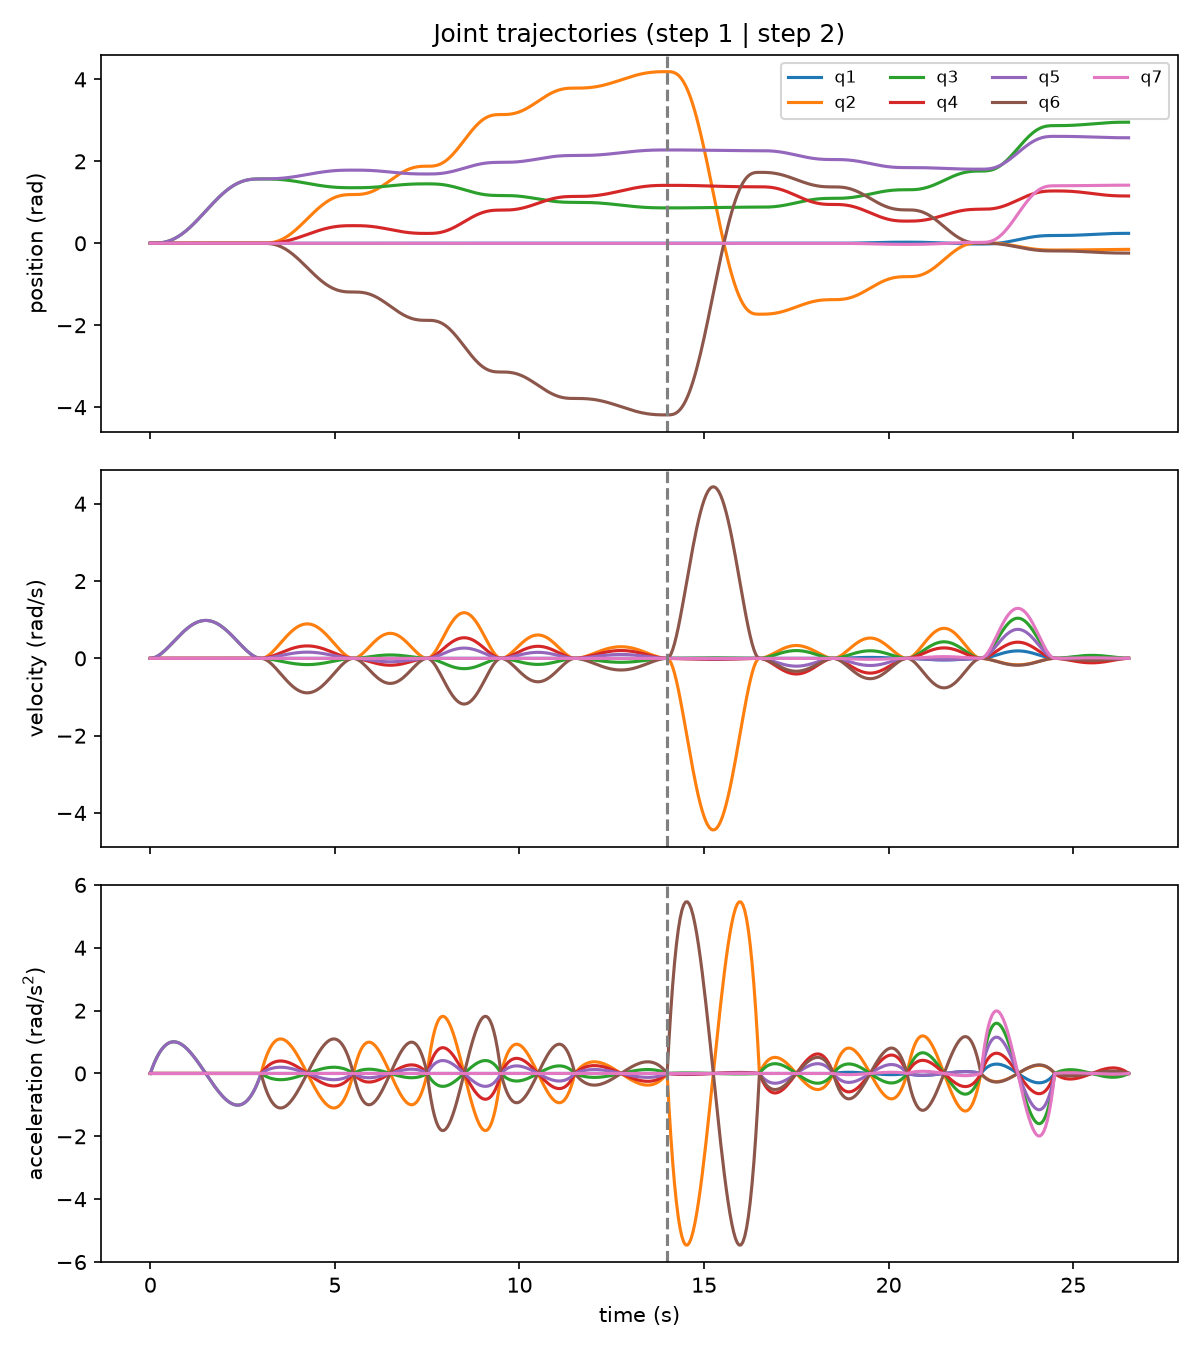
\includegraphics[width=0.85\textwidth]{joint_curves.png}
  \caption{关节位置/速度/加速度曲线}
  \label{fig:curves}
\end{figure}

\begin{figure}[htbp]
  \centering
  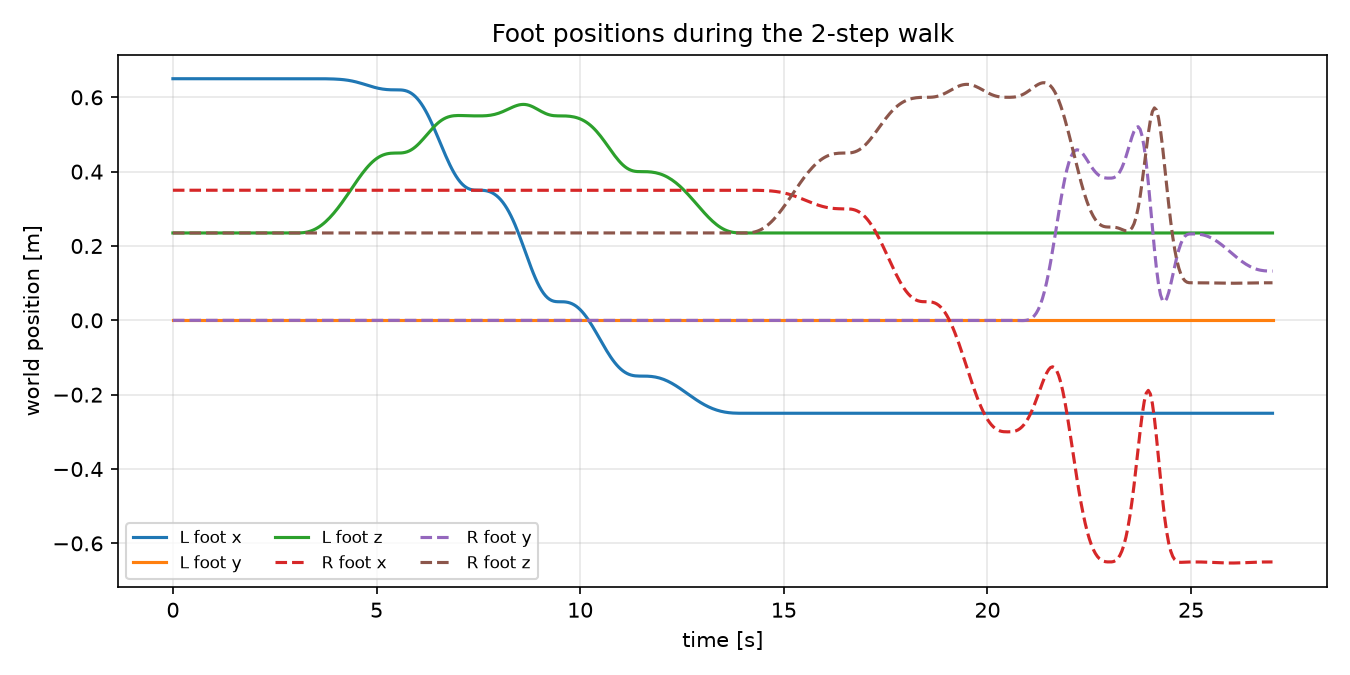
\includegraphics[width=0.85\textwidth]{foot_positions.png}
  \caption{两足端位置随时间变化曲线}
  \label{fig:feet}
\end{figure}

\end{document}
